\section{Result: Standard Network}  \label{s:N_II:std_net}

\vspace{3mm}
% \noindent\rule{17cm}{0.2pt}
\fbox {
    \parbox{\linewidth}{
      \begin{itemize}
        \item New Abs-Ca and P0 splits
        \item Characterisation of the the communities based on the tissue differentiated status
        \item 
      \end{itemize}
    }
}
\vspace{3mm}

% Non-tum split
\subsection{Non-tumour split} \label{s:N_II:std}

% Introduction to the work
The non-tumour dataset consists of three different tissue types: undifferentiated (UD), AbsCa-differentiated (Abs-Ca) and P0; see \cref{s:lit:datasets_used}. To further test the new version of the network pipeline it was used to stratify the non-tumour dataset with the goal to check if it finds the three groups of samples. 

% Introduce the methods used to get the groups
To achieve this, the same filtering as in \cref{s:cs:pre-processing}, is it used to select the 5000 most varied genes, then the network pipeline is applied. The output which consists of the MEVs was then analysed with both the cluster analysis described in \cref{s:cs:methods} and the Morpheus \ref{}. Due the small number of samples (88) the Morpheus software was preferred to visualise and perform the hierarchical clustering, with average linkage and cosine distance. Applying quantile normalisation on the dataset aid the visualisation of the heatmap and resulted in \cref{fig:N_II:morph_non_tum}. There are four metadata shown at the top of the figure: 
\begin{itemize}
    \item gender: Male (M), F (Female)
    \item \acrfull{nhu}: Abs-Calcium (Abs-Ca), undifferentiated (UD) and in-situ (P0)
    ABS-Ca, P0, UD)
    \item subset name: Bladder differentiated (B-Diff), (NR-DIF), Urothelium differentiated (Uro-D), P0 (Uro-P0) and undifferentiated (Uro-UD)
    \item diagnosis - \acrfull{ic}, \acrfull{cc},  , \textbf{nsUI (?)},  \acrfull{nvh}, \acrfull{oab}, Prolapse, \acrfull{ruti}, \acrfull{sui}
\end{itemize} 

% Heatmap -
From the heatmap in \cref{fig:N_II:morph_non_tum} it can be seen that the hierarchical clustering finds the three distinct groups of tissue differentiation, which further validates the approach. On top of that, as the dendrogram cut is increased to 7, there are other subgroups: a male subtype by cluster 5 and two main subtypes of the differentiated samples (6 and 7); see \cref{fig:N_II:sankey_comp}. The P0 subgroups are also split into two if the dendrogram cut is further increased, while there are 3 P0 samples which are clustered differently from the rest of the P0 samples. 

\begin{figure}[!htb]    
    \centering
    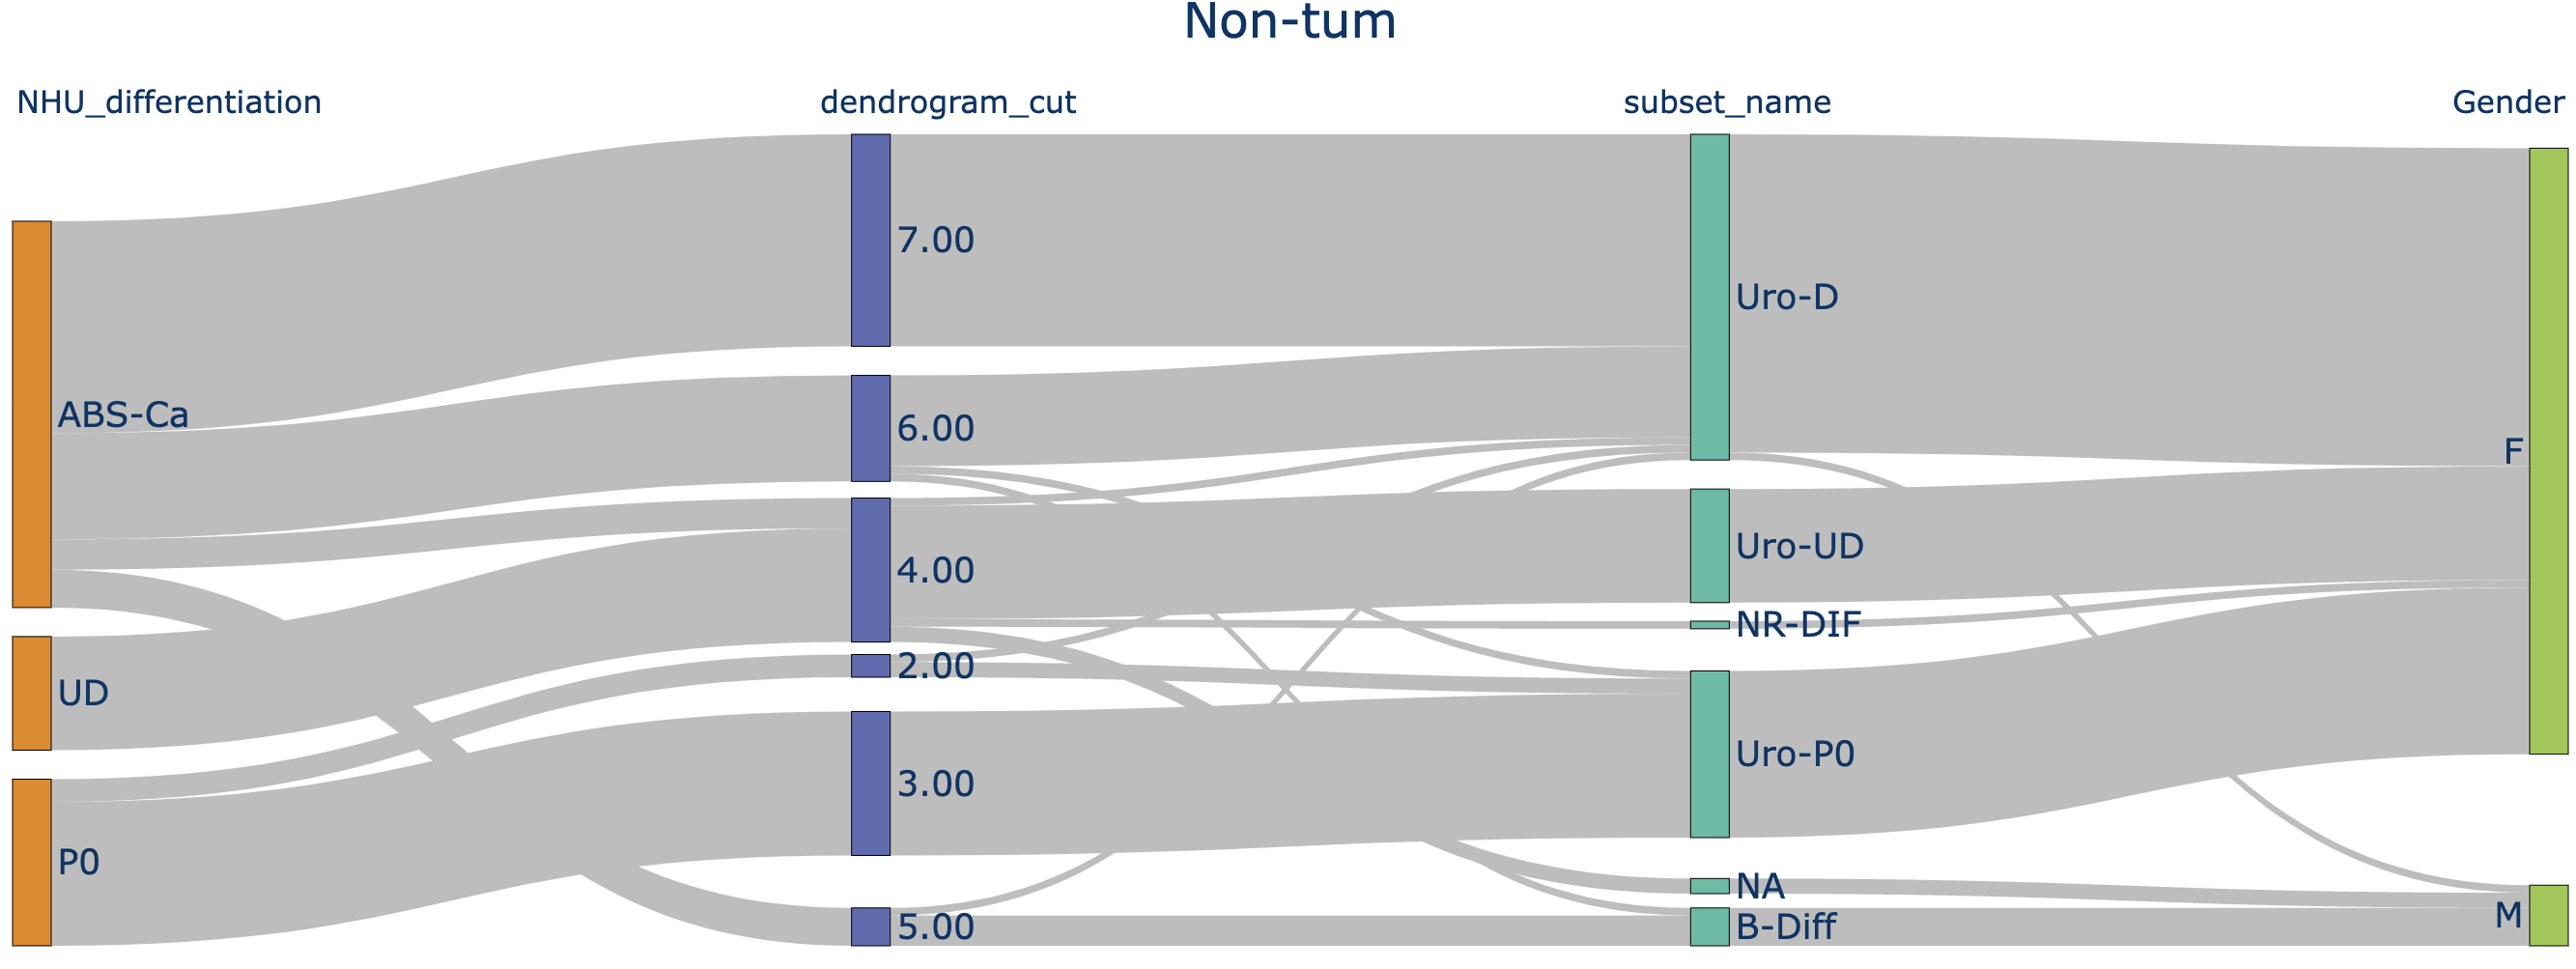
\includegraphics[width=1.0\textwidth,height=1.0\textheight,keepaspectratio]{Sections/Network_II/resources/non_tum/non_tum_split.png}
    \caption{Sankey plot that shows the non-tumour dataset split compared with the NHU differentiated status, subset and gender. It shows that the new network pipeline can find the three distinct differentiated tissues.}
    \label{fig:N_II:sankey_comp}
\end{figure}

% Explain the P0
The three 'isolated' P0 samples: Y2306, Y2439 and Y2383 had a high immune response which was highlighted by \textbf{...}. The male predominant group (5): Y815A-Bl, Y836B-Bl, Y499B-Bl, Y929B-Bl are paediatric samples which may explain why were grouped. However, Y719B-Bl is also a male paediatric sample but was grouped with the large differentiated subtype (7); see the only male sample on the right hand side of the heatmap. \acrfull{dea} and \acrfull{gsea} was used to determine if there are any chromosome Y specific signatures in this group but without any success; see \cref{appendix  for this}.

% Talk about the male differentiated samples that are pedriatic
The Abs-Ca samples are split into a smaller (14 samples) and a large (28 samples) group; see \cref{fig:N_II:sankey_comp}. From inspecting the heatmap, \cref{fig:N_II:morph_non_tum}, the smaller differentiated group is enriched in communities 19, 1 and 29 while the large group is not. Group 7 (large group) is also enriched in communities 25 and 22,  but 6 (smaller group) has a low expression of these communities. This means, that enrichment in communities 19, 1, 29, 25 and 22 establish the differences between the two differentiated groups. This is further explored in \cref{s:N_II:diff_split}.

% P0 difference
The difference in P0 is not as evident as in the Abs-Ca samples split, but it can be seen that the smaller P0 group is enriched in 25 while the larger P0 is less so. In addition, the genes from community 19, 29 are more expressed in the larger P0 group compared to the smaller subtype. This indicate that communities 25, 19 and 29 play a role in making the difference. The difference in the P0 samples are further explored in \cref{s:N_II:p0_split}.


% \begin{figure}[H]    
%     \centering
%     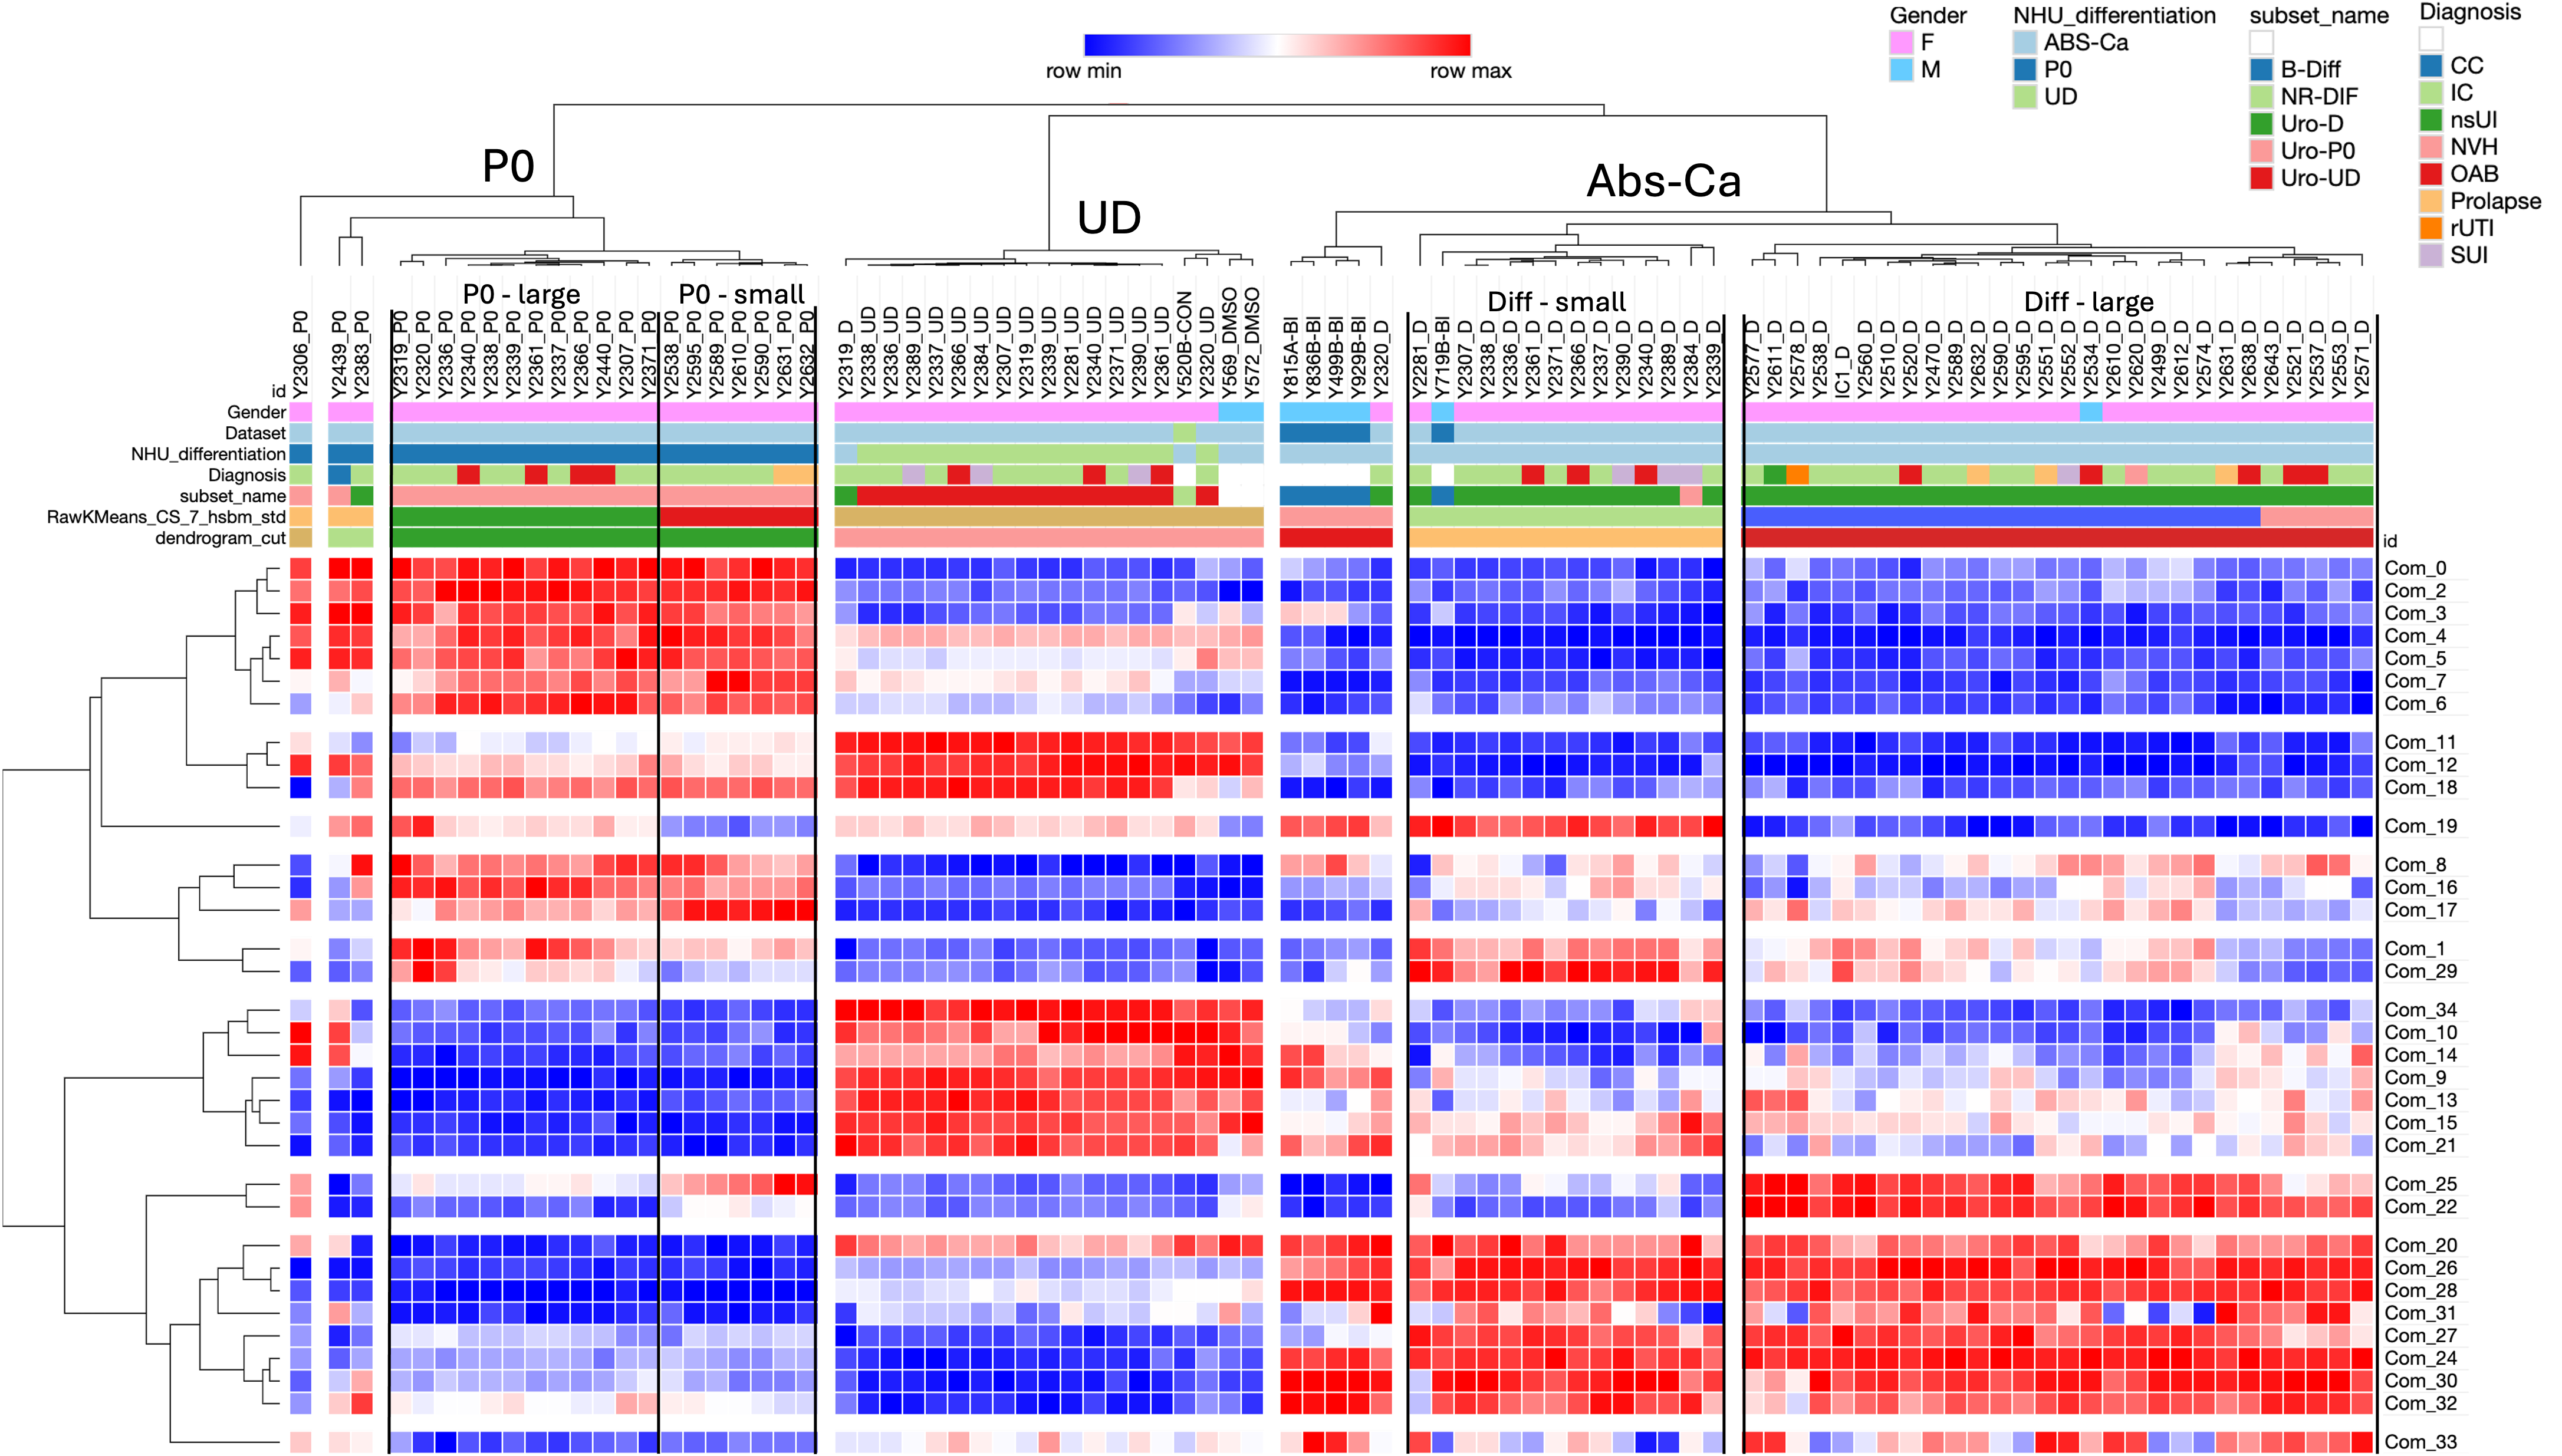
\includegraphics[width=1.0\textwidth,height=1.0\textheight,keepaspectratio]{Sections/Network_II/resources/non_tum/norm_healthy_std_3.1.png}
%     \caption{Heatmap showing both the groups in the non-tumour dataset and the clustered communities. Hierarchical clustering with average linkage and cosine distance is applied on the MEVs resulted from the network pipeline. There are four metadata shown at the top: Gender, NHU differentiation, subset name and the Diagnosis. }
%     \label{fig:N_II:morph_non_tum}
% \end{figure}


\begin{figure}[H]
    \centering
    \begin{minipage}[t]{1.0\textwidth}
        \centering
   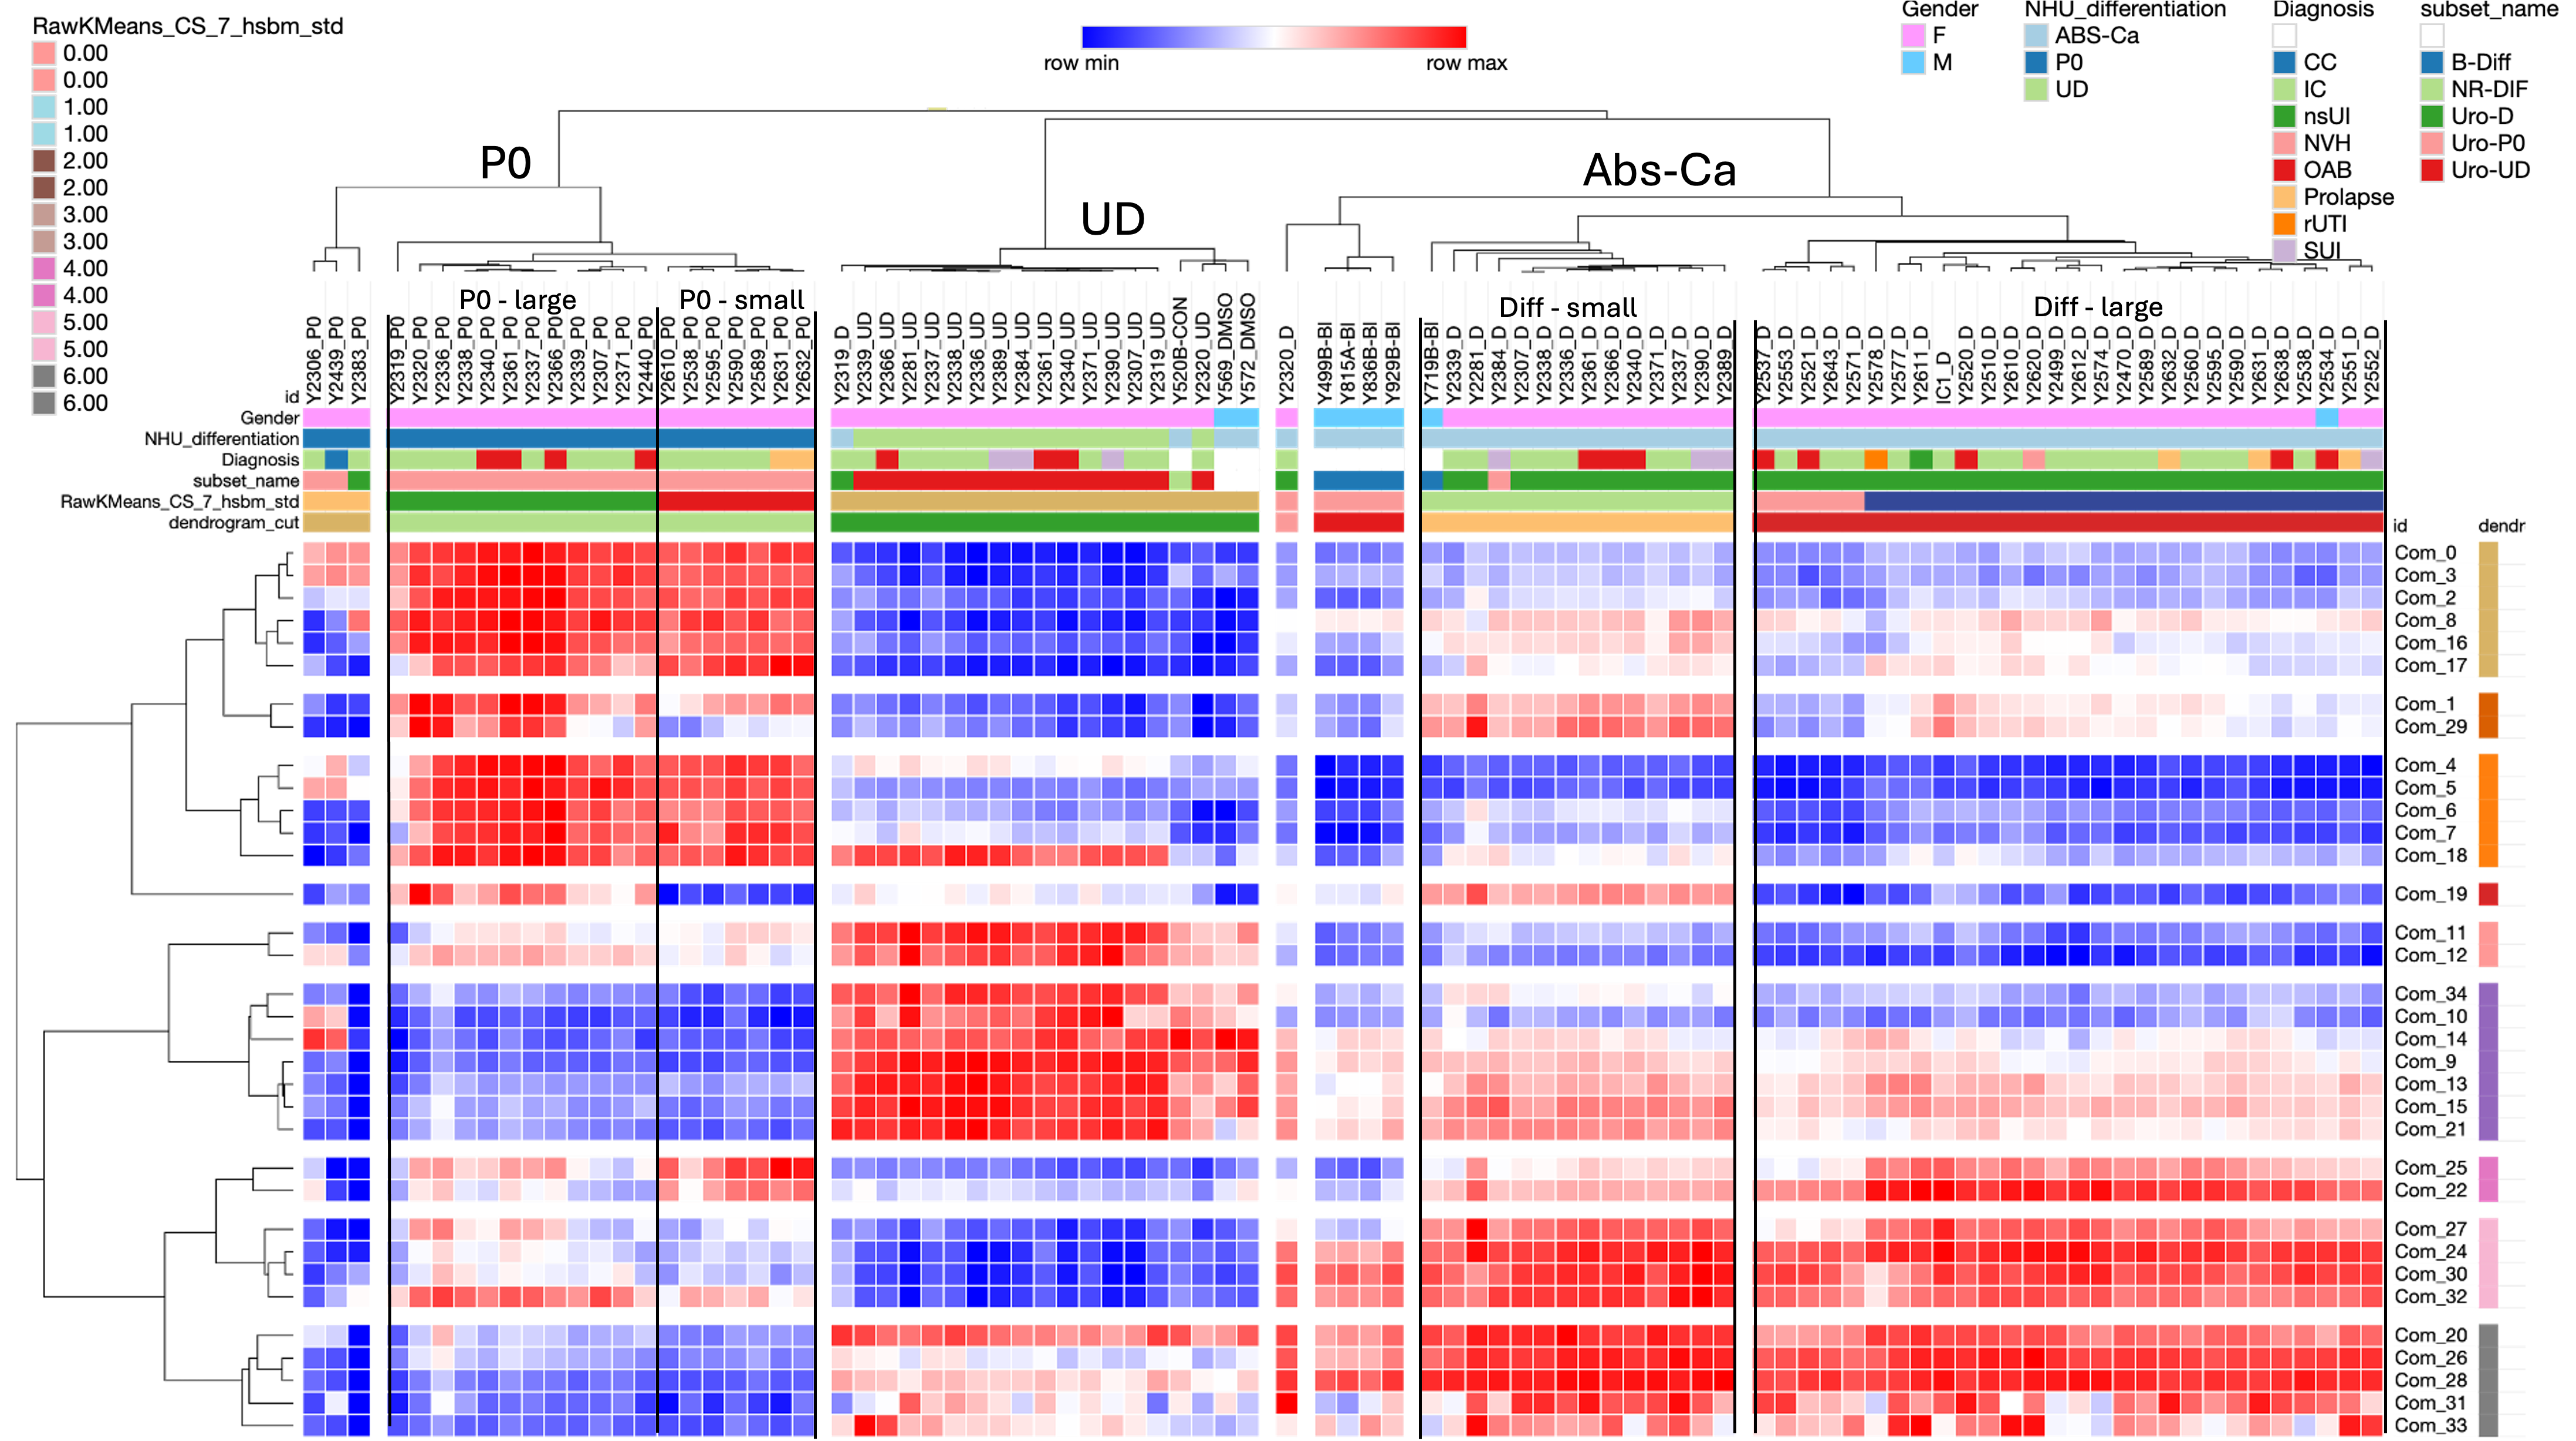
\includegraphics[width=1.0\textwidth,height=1.0\textheight,keepaspectratio]{Sections/Network_II/resources/non_tum/rotated_healthy_std_3.1.png}

    \end{minipage}%
    \begin{minipage}[b]{0.2\textwidth}
        \centering
        \rotatebox{90}{
        \begin{minipage}{\textheight}
        \caption{Heatmap showing both the groups in the non-tumour dataset and the clustered communities. Hierarchical clustering with average linkage and cosine distance is applied on the MEVs resulted from the network pipeline. There are four metadata shown at the top: Gender, NHU differentiation, subset name and the Diagnosis. }
        \end{minipage}
        }
    \end{minipage}
    \label{fig:N_II:morph_non_tum}
\end{figure}



% Abs-Ca splits
\subsection{Abs-Ca splits} \label{s:N_II:diff_split}

% Introduce the Splits
Both the heatmap (\cref{fig:N_II:morph_non_tum}) and Sankey plot (\cref{fig:N_II:sankey_comp}) show that the Abs-Ca differentiated samples are split into three different subtypes: 5, 6, and 7. It was mentioned earlier that group 5 consists of paediatric samples, which could explain the separation. To further explore the differences between groups 6 (small Abs-Ca) and 7 (large Abs-Ca), \acrfull{dea} was performed between the samples using the same method as in \cref{method for DEA}.


% Describe the DEA
The results of the \acrshort{dea} can be seen in \cref{s:N_II:diff_split}, where the X-axis represents the difference in gene expression ($log_2(\text{fold\_change})$), while the Y-axis shows the significance of the change given by $-log_{10}(q)$. As the name suggests, "Point(s) of interest" are the genes that are outside of the $log_2(\text{fold\_change})$ bounds (\textbf{$+/-1$ - check}) and have a high expression difference, making them worth considering for future analysis. The 'Dataset' includes all the other points common to both groups. The '19', '1', '29', '25', and '22' coloured points represent the genes selected by ModCon for each respective community.

% Analysis of the volcano plot
In \cref{fig:N_II:diff_split}, the left-hand side represents the genes that are highly expressed in the larger Abs-Ca group, while the right-hand side shows the genes specific to the small Abs-Ca group. From left to right, it can be noticed that the genes selected by communities 25 (green) and 22 (purple) are specific to the larger Abs-Ca group, which is highlighted by the heatmap in \cref{fig:N_II:morph_non_tum}. However, some of the genes in community 25 do not have a much higher expression in the large Abs-Ca group, as they are closer to the middle. On the other side, genes specific to community 19 are specific to the smaller Abs-Ca group. Genes from communities 29 and 1 are more expressed in the small Abs-Ca group but are at the threshold level of not having a high expression difference.

\begin{figure}[!b]    
    \centering
    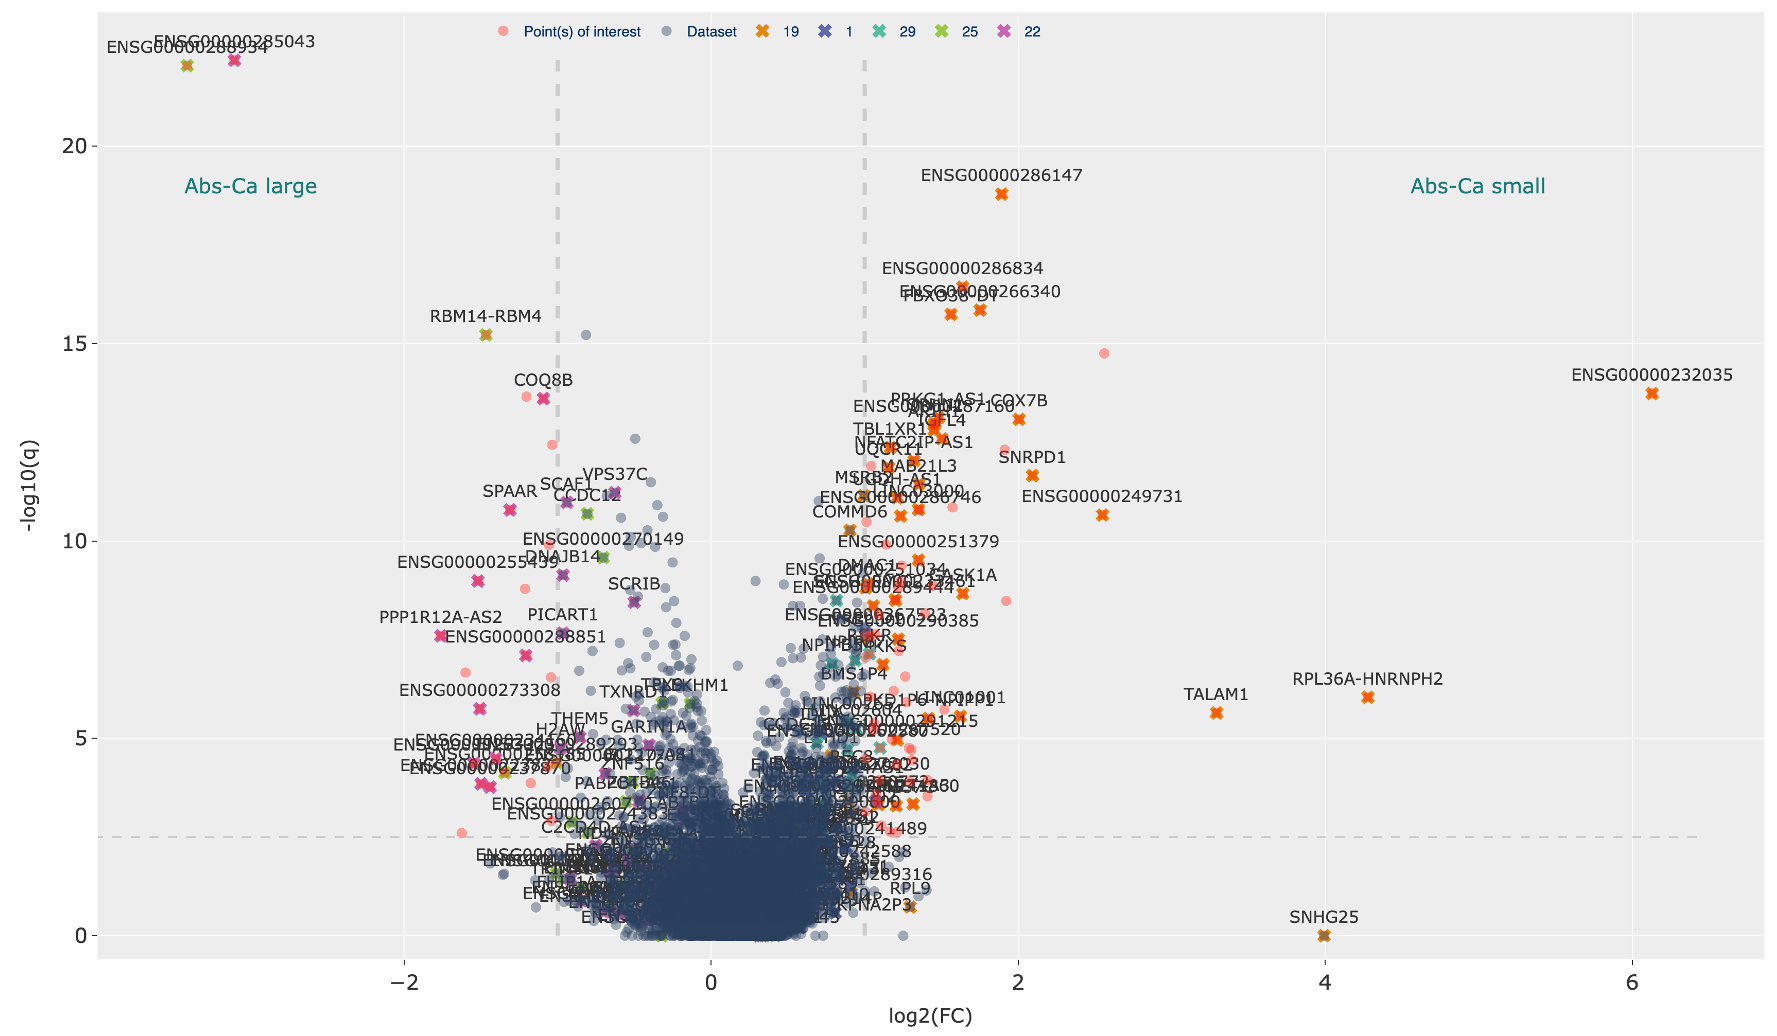
\includegraphics[width=1.0\textwidth,height=1.0\textheight,keepaspectratio]{Sections/Network_II/resources/non_tum/diff_split_dea.png}
    \caption{Volcano plot showing the \acrfull{dea} for the comparison between groups 6 (small Abs-Ca) and 7 (large Abs-Ca). The X-axis represents the difference in gene expression, $log_2(\text{fold\_change})$, while the Y-axis shows the significance of the change given by $-log_{10}(q)$. The genes on the right-hand side of the plot are those significantly expressed in the larger Abs-Ca group, while the points on the left-hand side are specific to the smaller Abs-Ca group.}
    \label{fig:N_II:diff_split}
\end{figure}

% Concluding analysis
The analysis suggests that the up-regulation of genes from community 19 is specific to the smaller Abs-Ca group, while the genes from community 25 are specific to the larger Abs-Ca group. Communities 29 and 1 have a 'tendency' towards the smaller group, while community 22 tends towards the larger group.

% Linking to the network and communities
It is remarkable that the network pipeline, through the ModCon score, is able to select most of the genes that are significantly different between the two groups. It is worth considering that the DEA uses all the expressed genes, while the network approach considers only 5000 genes. This demonstrates that the pipeline is capable of finding significantly different genes, which can also be linked to network communities.

% Talk about ENSG
Another important observation of the selected points in the volcano plot from \cref{fig:N_II:diff_split} is that many of the highlighted genes do not have assigned names, i.e., they follow the pattern 'ENSG...'. This indicates that many of the genes are unknown and have the potential to reveal new biological insights. However, this also means that these genes are challenging to study.



% P0 split
\subsection{P0 split} \label{s:N_II:p0_split}

% Why doing the P0
In the heatmap from \cref{fig:N_II:morph_non_tum} there is another split of a major differentiated tissue type, P0. This is not as clear as the Abs-Ca groups, but nevertheless present and it can be observed that communities '19', '22', '25' and '29' are driven the separation. To study more the division in the P0 samples, the same approach was taken as in the precedent sub-section, where \acrshort{dea} is applied and the genes selected through ModCon are highlighted in the plot.

% Introducing the volcano plot
The figure \cref{fig:N_II:p0_split} represents the resultant volcano plots between the two P0 subgroups, labelled as P0 large and P0 small. The genes on the left-hand side of the plot are higher expressed in the larger group and as higher these are on the Y-axis the more significant differentially expressed are. Conversely, on the right hand side are the genes representative for the smaller P0 group.

% Talk about the communities
The volcano plot confirms that the genes from communities 19 and 29 are up-regulated in the larger P0 but not expressed in the other group. Conversely, the expression of genes from 25 and 22 are more present in the smaller P0 compared to the larger subtype. It can also be noticed that most of the genes highlighted are predominantly "ENSG..." denoting the novelty of the findings but also the challenge of determining their function. 

This analysis reinforce the fact that the network pipeline is capable of finding communities which drive separation in well-known groups. It also shows that ModCon extracts genes that are significantly expressed in the group division.


\begin{figure}[H]    
    \centering
    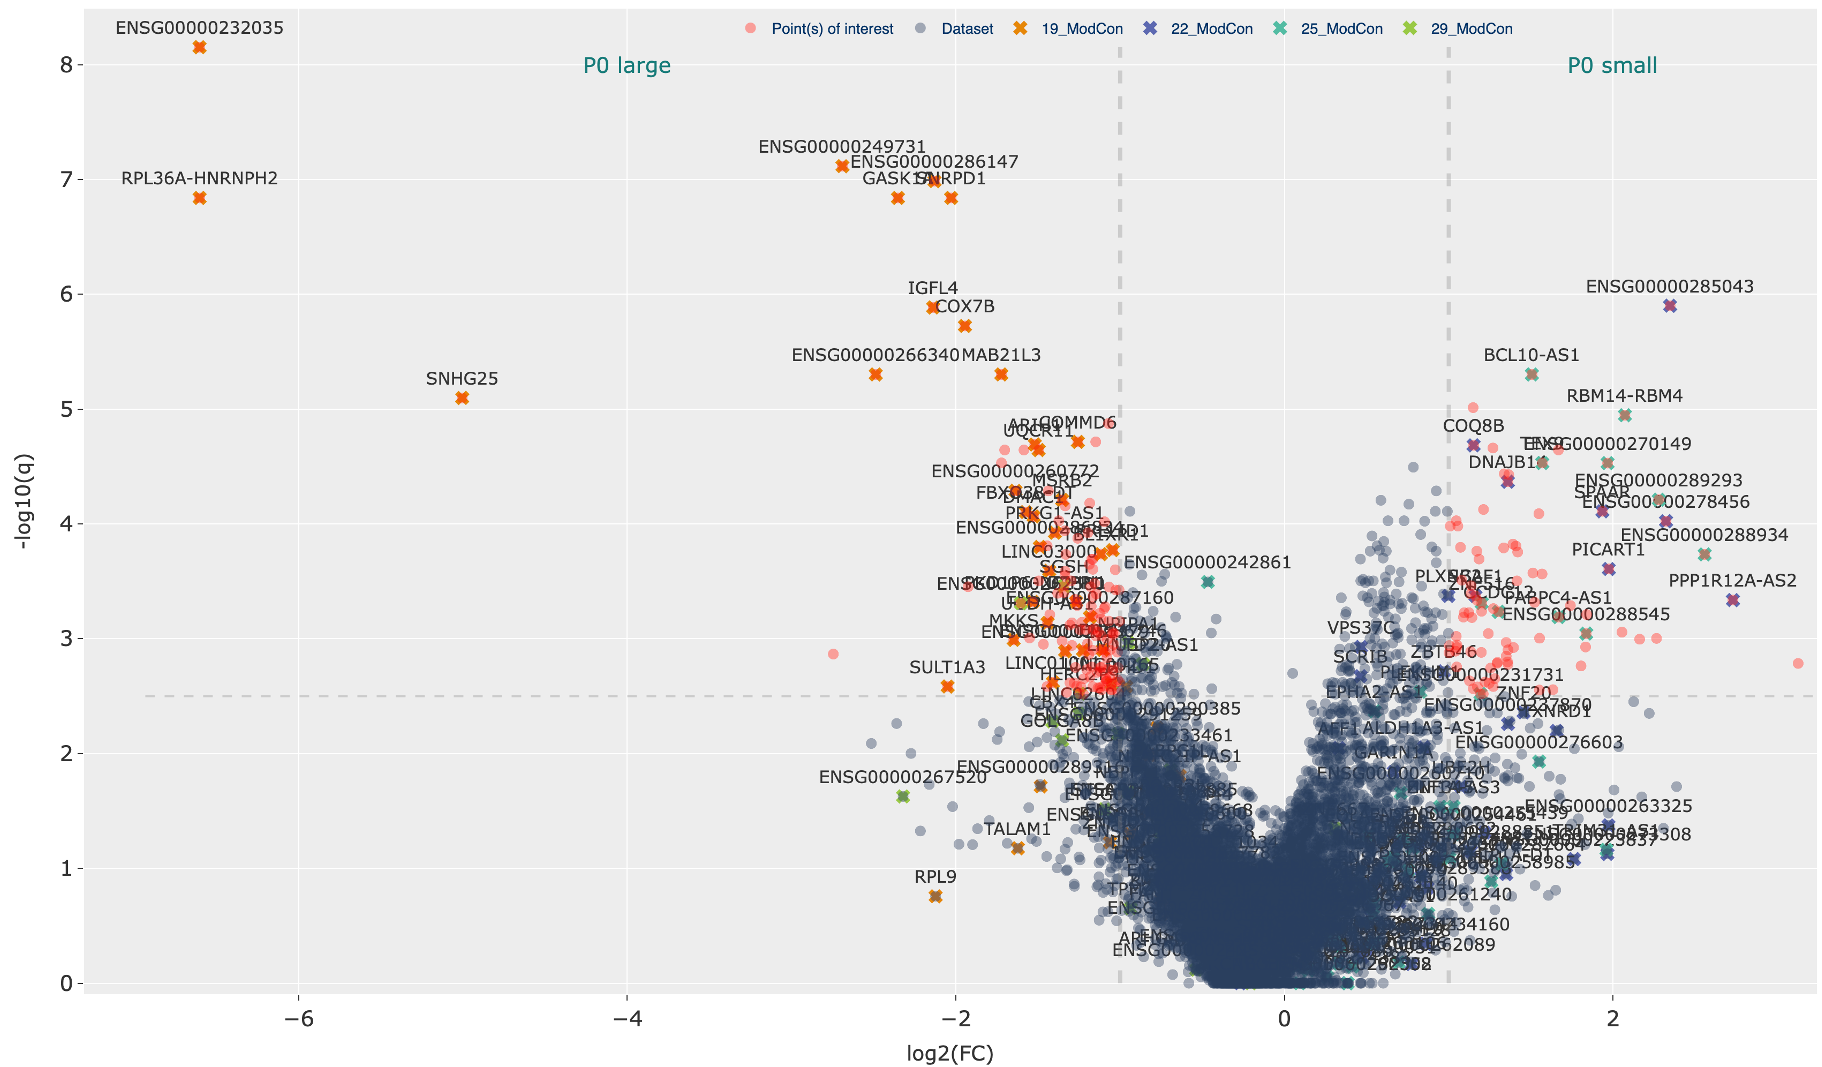
\includegraphics[width=1.0\textwidth,height=1.0\textheight,keepaspectratio]{Sections/Network_II/resources/non_tum/p0_split_dea.png}
    \caption{Volcano plot showing the \acrfull{dea} for the comparison between the P0 split shown in the heatmap from \cref{fig:N_II:morph_non_tum}. The X-axis represents the difference in gene expression, $log_2(\text{fold\_change})$, while the Y-axis shows the significance of the change given by $-log_{10}(q)$. The genes on the right-hand side of the plot are those significantly expressed in the larger P0 group, while the points on the left-hand side are specific to the smaller P0 group.}
    \label{fig:N_II:p0_split}
\end{figure}




% Community characterisation
\subsection{Community characterisation} \label{s:N_II:comm_charact}

% Talking about the significance of the finding
In the two cases of the P0 and Abs-Ca splits, it can be observed which communities are driving the separation. It can also be noticed that the genes in these communities are found to be significantly expressed when performing the \acrlong{dea}. These two results have a two-fold implication. First, the network pipeline, and implicitly the hierarchical SBM, is able to find communities that are significantly expressed in some groups, demonstrating the power of the method. Secondly, the splits in the Abs-Ca and P0 samples indicate the opportunity to further explore new biological aspects of the differentiated status.

% Talk about the misfit communities
From the heatmap (\cref{fig:N_II:morph_non_tum}) and the two volcano plots (\cref{s:N_II:diff_split,fig:N_II:p0_split}), it can be noticed that a few communities have a stronger influence on the splits. Communities 19 and 29 are specific to the small Abs-Ca and the small P0 groups, while community 25 is specific to the large Abs-Ca and small P0 groups. It can be seen in the clustering of the communities in \cref{fig:N_II:morph_non_tum} that these are clustered separately or with weaker communities (1 and 29, and 25 and 22).



\begin{figure}[H]    
    \centering
    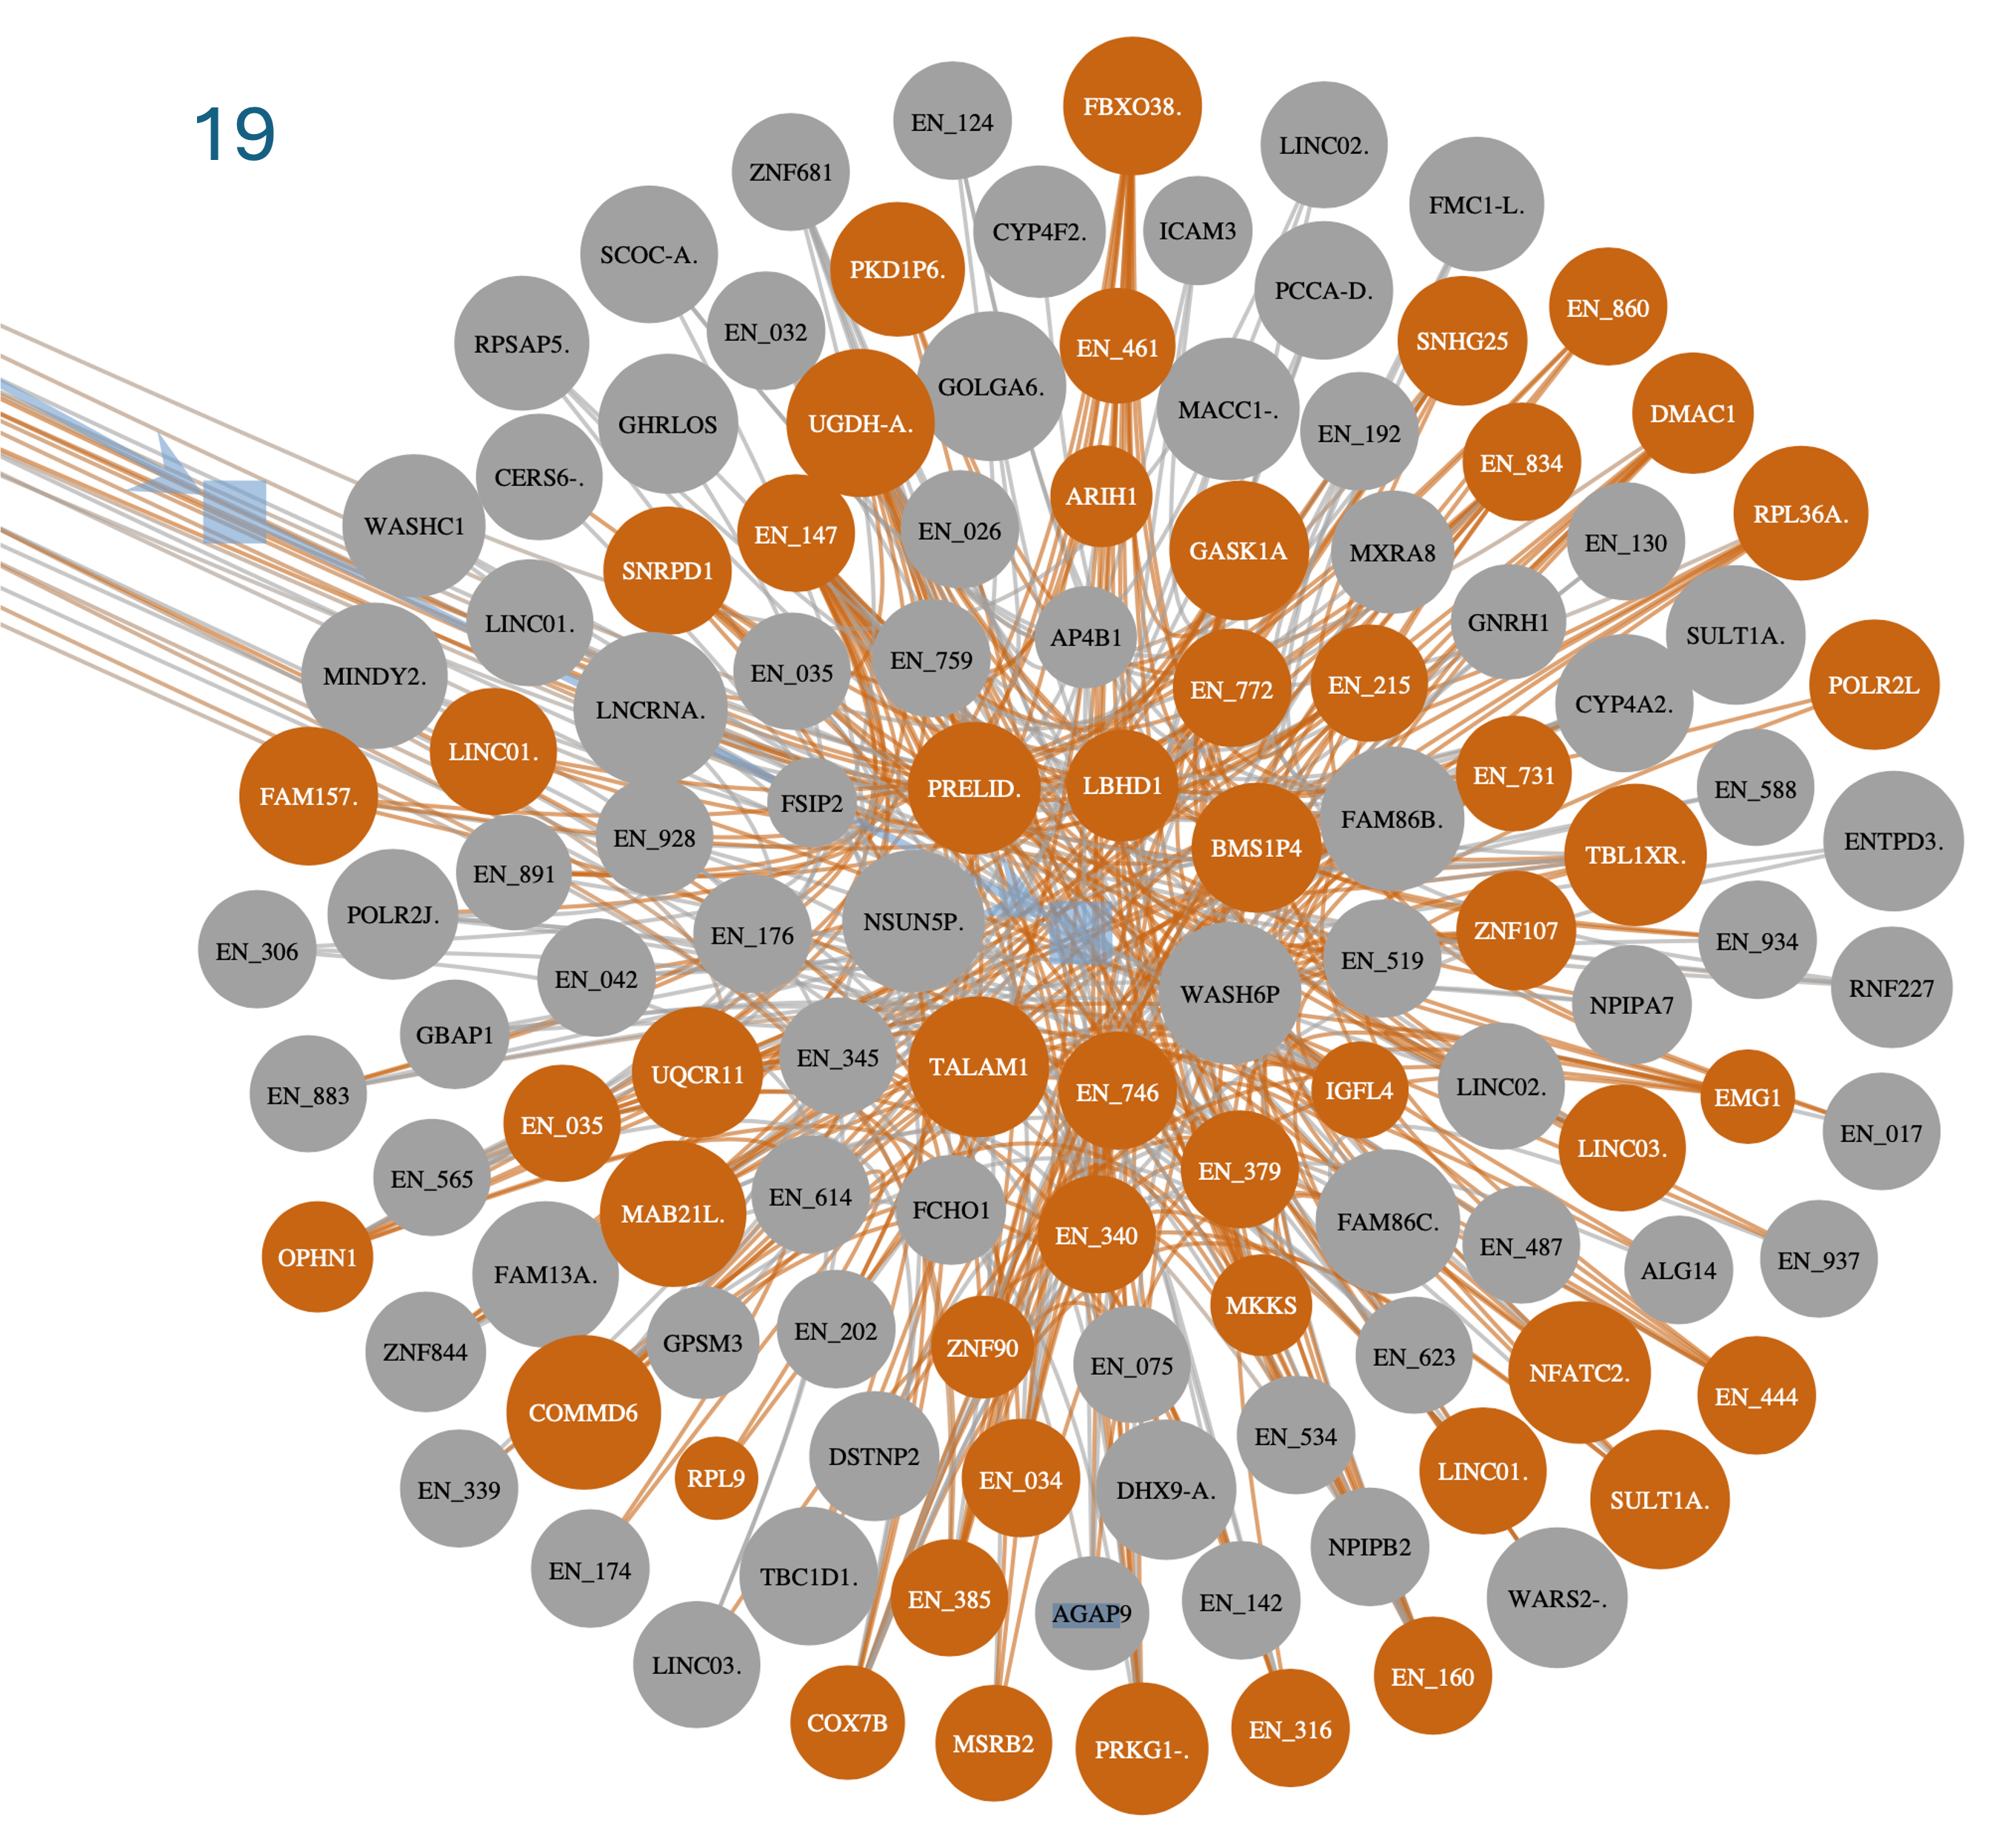
\includegraphics[width=1.0\textwidth,height=1.0\textheight,keepaspectratio]{Sections/Network_II/resources/non_tum/19_com.png}
    \caption{Community 19 from the standard network generated from 5000 genes, no weight modifier and to which the \acrshort{hsbm} was applied. The community contains 123 genes from which 50 with the highest ModCon score are highlighted in orange. To aid the visualisation some of the genes were trim, for the ones with longer names the first 5 letters were kept while for 'ENSG...' like nodes the "EN\_" and the last 3 digits were kept. }
    \label{fig:N_II:19_com}
\end{figure}


% Linking the Volcano plots with the network.
Community 19 seems to be the leading driver of the splits, and to showcase the visualisation aspect of the networks, the genes forming the group are shown in \cref{fig:N_II:19_com}. The module comprises 123 genes, with the genes coloured in orange being the 50 with the highest ModCon scores\footnote{Note that there are 100 genes selected for the MEVs, but only 50 are highlighted in the community to ease visualisation.}, some of which were significantly expressed in the Volcano plots from earlier. In the case of the Abs-Ca split, genes like \textit{TALAM1}, \textit{SNRPD1}, \textit{COX7B}, or even \textit{ENSG0000023205} are in the top 50 ModCon. For the P0 split, nodes like \textit{SNHG25}, \textit{IGFL4}, \textit{MAB21L3}\footnote{Gene \textit{MAB21L3} is trimmed to \textit{MAMB21L} in the network as part of the automatic process to shorten the longer genes and help with visualisation}, and again \textit{ENSG0000023205}. The connection between ModCon and the genes found through the DEA affirms the utility of using the network and its usefulness to analyse subsets of genes. Similar analysis was performed for communities 25 and 29, which can be found in \cref{ap:N_II:coms} from the Appendix.



% Community characterisation
Apart from the differences in the P0 and Abs-Ca samples, the heatmap shows that the communities can be labelled as tissue-specific. For example, communities 0, 2, 3, 4, 5, 7, and 6 are all more enriched in the P0 samples, while communities 11, 12, 34, 10, 14, 9, 13, 21 are enriched in the UD samples. Towards the bottom of the heatmap, communities 20, 26, 28, 31, 27, 24, 30, and 32 are enriched in differentiated tissue. Communities 19 and 29, which drive the Abs-Ca/P0 split, do not belong to any group and are classified as 'Misfit,' while community 18 is enriched in both UD and P0 samples.


% Why I am putting this here
Assigning them a tissue function may help in further analysis of the MIBC subtypes. To further validate them, DEA was performed between the three datasets: Abs-Ca, UD, and P0. For each community, the genes selected by ModCon (top 100) were plotted against the volcano plots, as in \cref{fig:N_II:p0_split,s:N_II:diff_split}. This allows for confirmation of the 'trends' in the communities. The results can be seen in the cluster tree in \cref{fig:N_II:cluster_tree}, generated using \citet{Zappia2018-bt}.

% Summary of the work
The cluster tree represents a summary of the work done in this section, where each community was labelled by their enrichment in the tissue-differentiated samples. The communities found at the lowest level (0) are also detectable with the standard SBM; the hierarchical version simply performs an additional clustering from bottom to top. This means that the communities from level 0 SBM are applied, resulting in the 14 communities at level 1, and this continues until there is one single community found, in this case, until level 4. All the analysis performed in this section is at level 0, and then the information is propagated upwards.

% Commenting on the cluster tree
It can be observed that at level three, there are different communities almost corresponding with the differentiated properties of the datasets used. It is not surprising to see that P0 and Abs-Ca (Diff) are grouped together as they are 'closer' on a differentiation spectrum. One can also notice that there is a difference in the grouping performed by the traditional hierarchical clustering in the heatmap from \cref{fig:N_II:morph_non_tum} and the SBM version in the cluster tree \cref{fig:N_II:cluster_tree}. This is because the hSBM uses all genes, while the standard hierarchical clustering receives the MEVs for a selected few via ModCon.


% Talk about the misfits and comment the clustertree

\begin{figure}[H]    
    \centering
    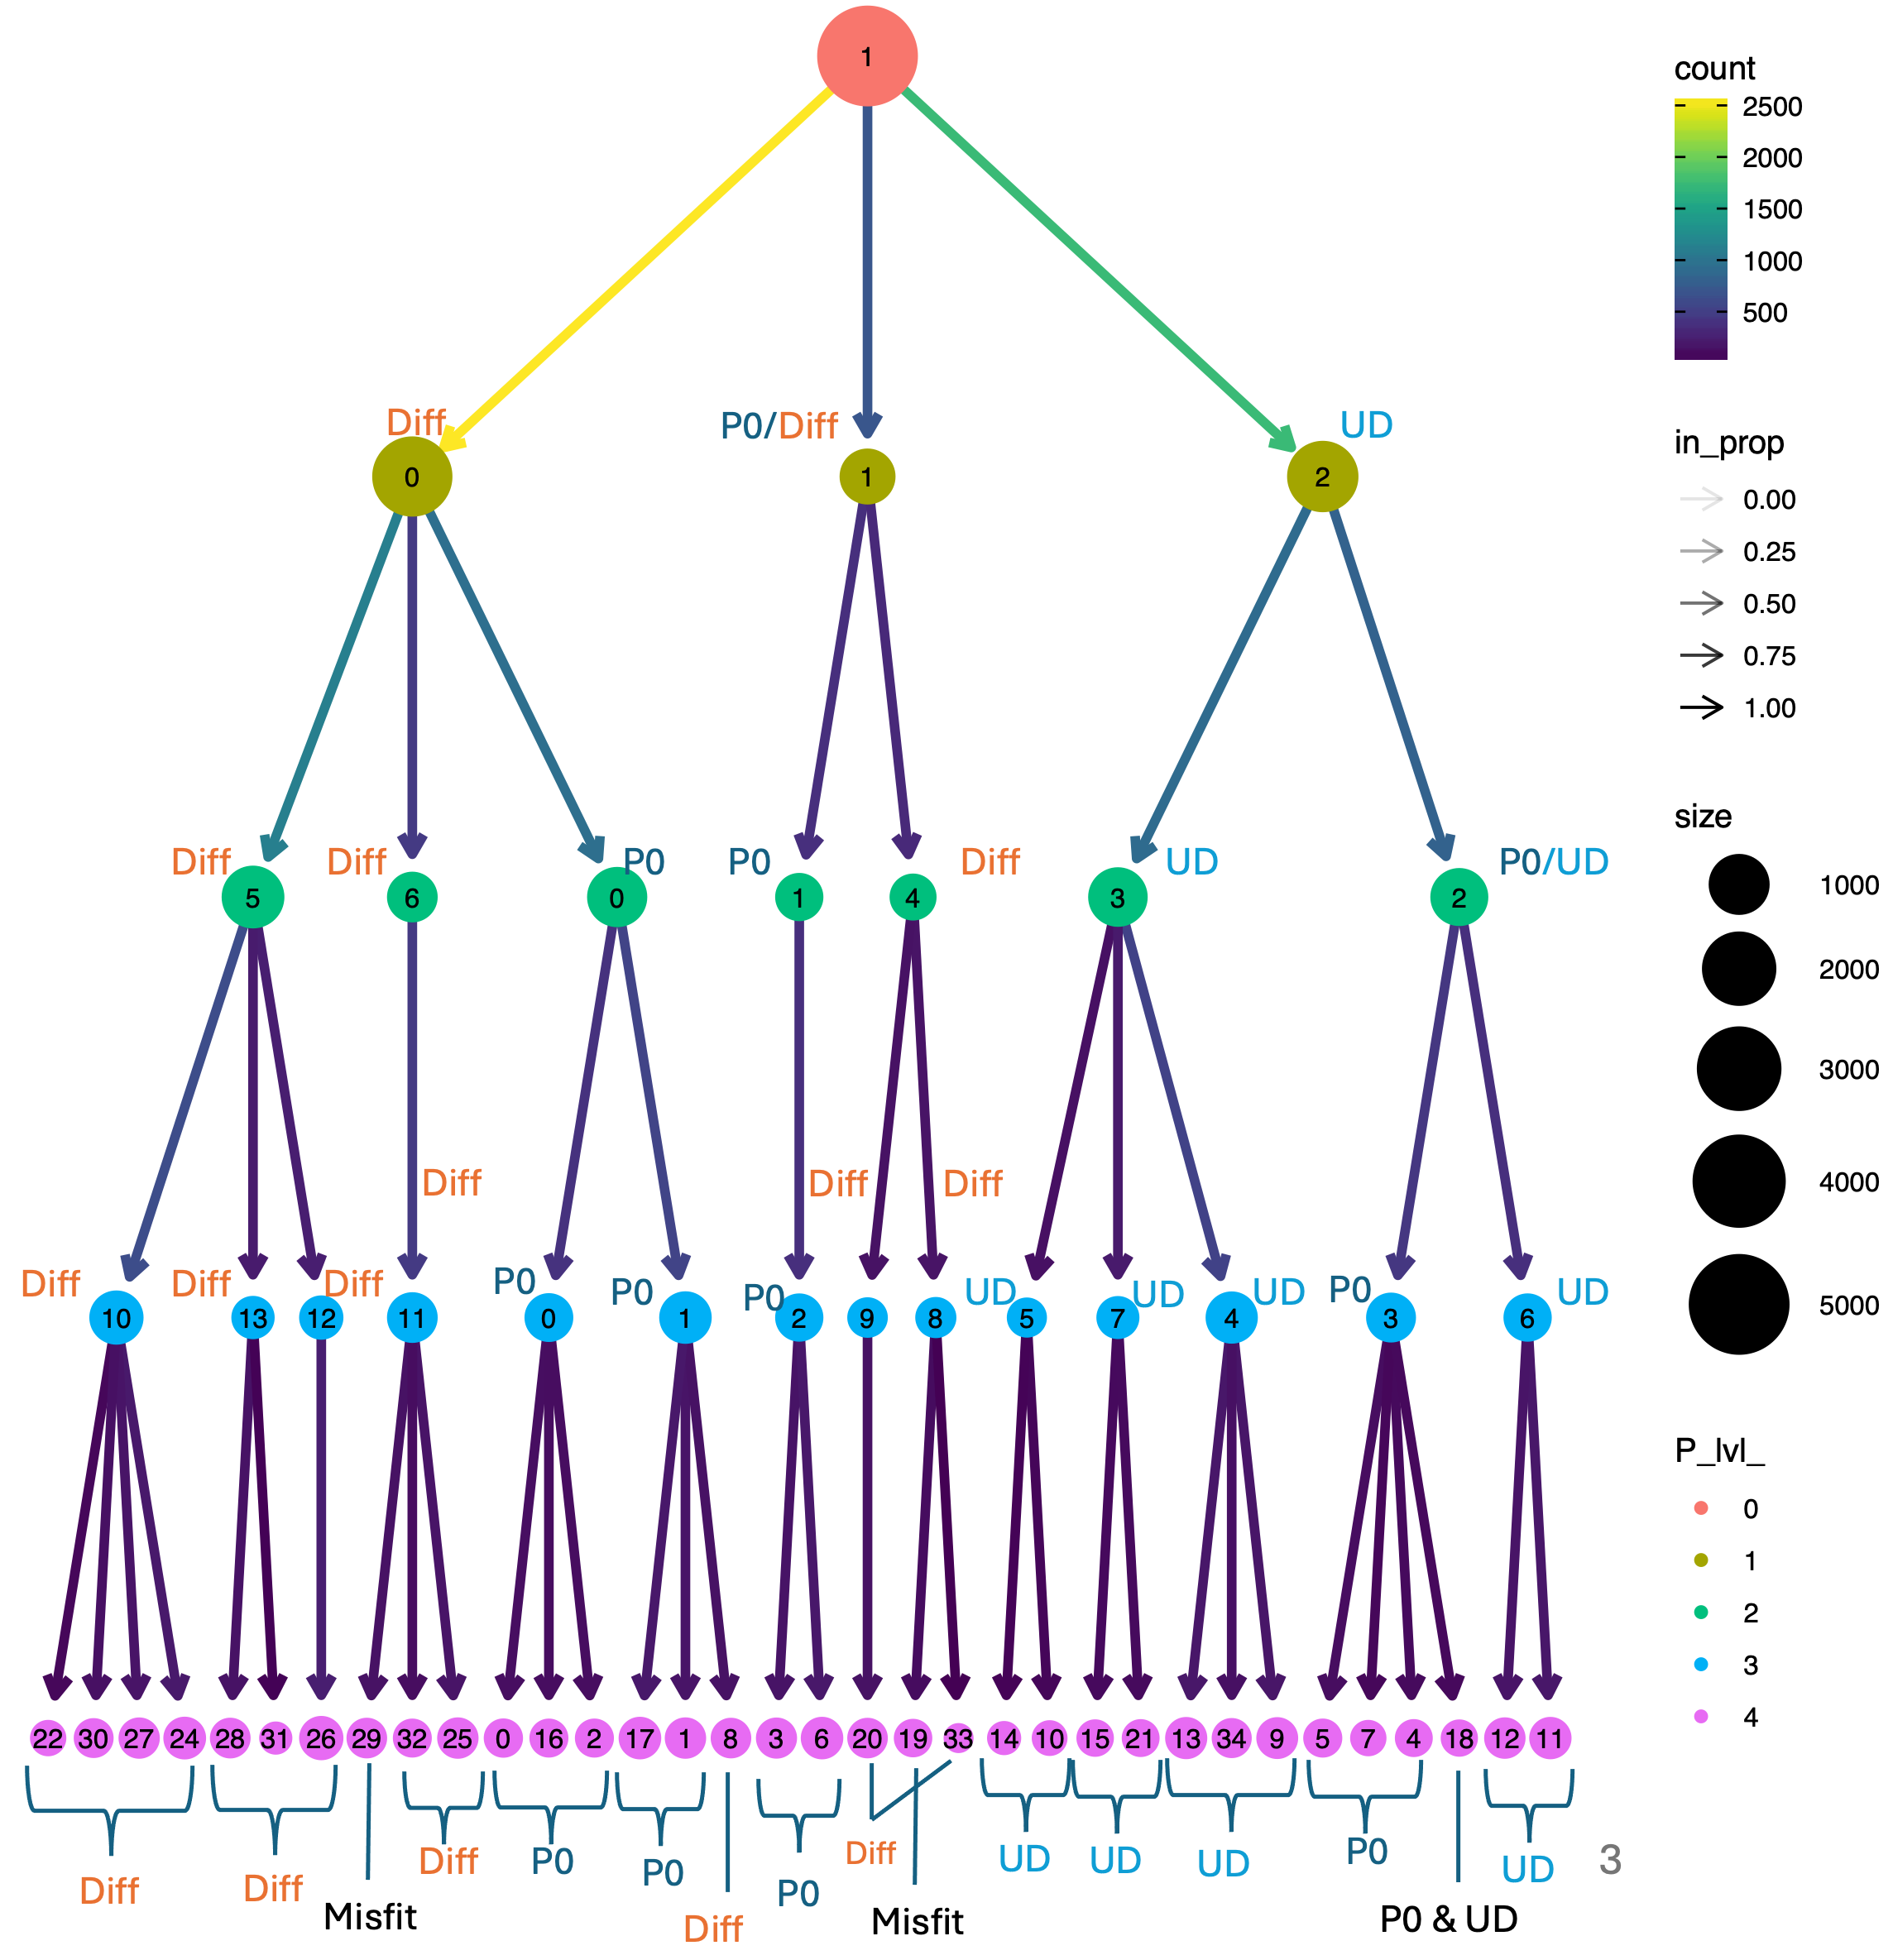
\includegraphics[width=1.0\textwidth,height=1.0\textheight,keepaspectratio]{Sections/Network_II/resources/non_tum/clustertree_labels.png}
    \caption{Cluster tree }
    \label{fig:N_II:cluster_tree}
\end{figure}



% 
\subsection{MIBC split} \label{s:N_II:tum_split}

% Introduce the work
The non-tumour stratification yield some new groups in two of the three datasets used to built the graph but how capable is the standard network to subtype the MIBC cohort from TCGA? This part of the chapter attempts to answer the question by using the same network presented earlier: 5000 most varied genes, 3 edges per standard gene and 6 per TF and using hierarchical SBM. The main difference is that the stratification is performed on the tumour rather then the non-tumour dataset. This means a different dataset is used from which the network was built and the integrative MEV (iMEV) presented in \cref{s:N_II:iMEV} is used.

% Describe the figure
The resultant MEVs are analysed with Morpheus \citet{broad}, \cref{fig:N_II:tum_morph}, which are first quantile normalised, then the hierarchical clustering with average linkage and cosine distance is applied. Dendrogram cuts of 10 for samples and 6 communities are used as higher values lead to more smaller communities (mostly of 1-2 samples). At the top is shown the classifications by the work presented in the first chapter \cref{s:cs:bio_interp}, TCGA \citet{Robertson2017-mg}, consensus\citet{Kamoun2020-tj} and Lund \citet{Marzouka2018-ge}. On the right hand side the "Diff Type" represents the community labelling from the last section.

% Talk about the splits
The heatmap in \cref{fig:N_II:tum_morph} demonstrates that MIBC is categorised into the two canonical groups: Luminal on the left (green by Consensus/TCGA) and Basal (mostly blue by Consensus/TCGA) on the right. The Luminal group is further divided into six subgroups, two of which consist of a few samples, and three larger groups. The remaining four clusters are Basal subgroups, with one group being particularly enriched in Stroma according to TCGA. Notably, there is no evidence of the three Basal splits by the \acrfull{ifn} response observed in the first part of the project, nor a distinct separation of a Mes-like group as discussed in the third chapter (\cref{s:N_I:sel_pruning}). Observing the top dendrogram, it is evident that as the cut increases, more groups emerge. A notable mention is the NE group on the left side of the Stroma group. However, artificially increasing the dendrogram cut does not enhance the outcome.

% Talk about the communities
Shifting the focus on the communities, the previous highlighted 19, 25 and 29 have a less clearer impact on the tumour stratification. These groups may be involved in the split of the luminal group \cref{fig:N_II:tum_morph}, but there are clearer communities that make the separation. For example, community 9, 13, 15, 21 classified as UD, are more enriched\footnote{By this I mean, the genes that are present in mentioned communities are more expressed in one group than the other} in the Basal than the Luminal groups while 8 (diff), 16 (p0), 17 (p0) are specific to the Luminal group and not to the Basal. Communities 1, 29, 25, 27 (diff) seems to be specific the Luminal group on the left-hand side with a low expression in all the Basal group. 

% Conclusion
The heatmap in \cref{fig:N_II:tum_morph} indicates that most of the diff and P0 communities are specific to the Luminal groups which are known to be closer to the healthy bladder differentiated tissue. While the UD modules are enriched in the Basal subtype which have an undifferentiated, squamous phenotype. However, there are a few exceptions , for example communities 4,5, 10, and 12 are generally enriched in all the samples apart from a few scatter across the heatmap the luminal group on the most left. Community 7 which was attributed P0 is hard to attribute a specific MIBC group, suggesting that it may contain genes expressed across all the subtypes.

Overall the analysis shows the potential of the network approach and using communities found in a non-tumour network and then used to stratify the MIBC. While these are not powerful enough the further stratify the MIBC in new groups, it shows that the communities can be used to focus the analysis. For example, one possible next step is to further investigate what are the genes in communities 4, 5, 10 and 12 as well as what makes the most left luminal community to be separated. However, due to the limited time in the PhD the efforts were concentrated on improving the reward modifier which is explored in the next section.


\begin{figure}[H]    
    \centering
    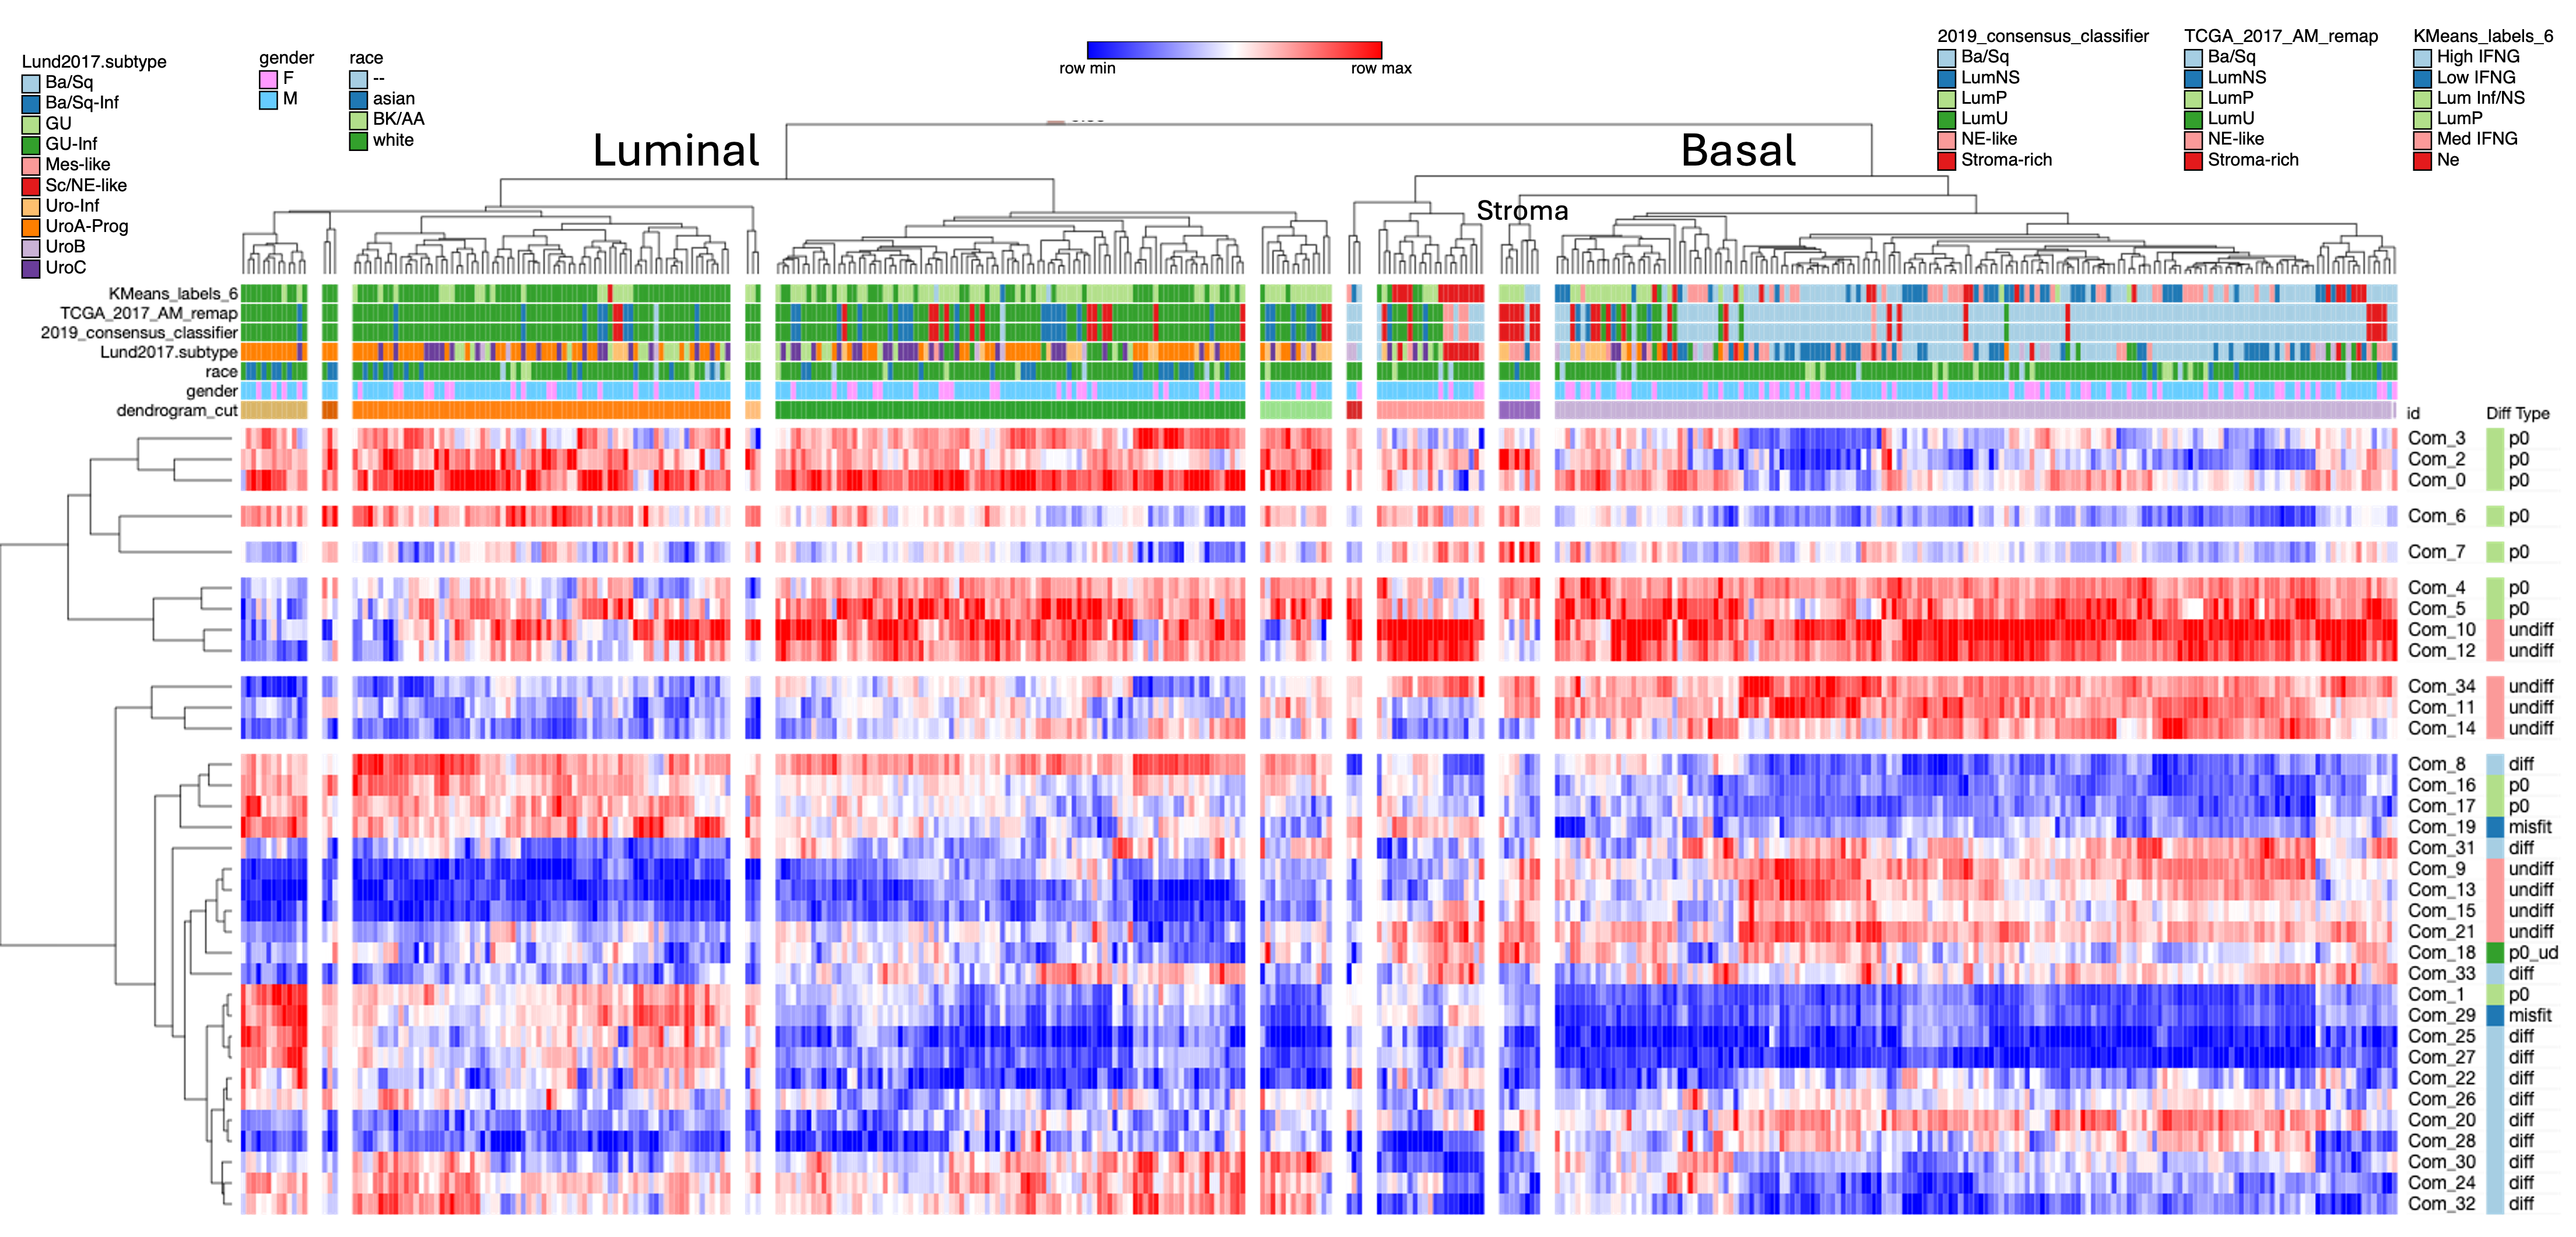
\includegraphics[width=1.0\textwidth,height=1.0\textheight,keepaspectratio]{Sections/Network_II/resources/non_tum/iMev_3_3_cs_13.png}
    \caption{Heatmap showing both the MIBC subtypes and the grouped communities by applying the hierarchical clustering with average linkage and cosine distance on the MEVs. There are four metadata shown at the top: gender (Female/Male), race (asian, black/afro-american and white), and the three referential classifier used in the project: Lund \citet{Marzouka2018-ge}, consensus\citet{Kamoun2020-tj}, TCGA \citet{Robertson2017-mg} as well as the work form the first chapter \cref{s:cs:bio_interp}. A dendrogram cut of 10 for samples and 6 for communities was used as higher values lead to more smaller communities. On the right hand side the "Diff Type" represents the community labelling from \cref{s:N_II:comm_charact}.}
    \label{fig:N_II:tum_morph}
\end{figure}



\subsubsection{Summary}

\begin{itemize}
    \item Talk about the opportunities to further split the P0 and Abs-Ca differentiated status 
    \item Link from the differentiated status to the communities and the hierarchical cluster tree
    \item This is a much smaller dataset then the TCGA and it shows that it is able to group samples based on the differentiated status - good validation
    \item Basal/Luminal subtype stratification's
    \item Novel split in the P0/Abs-Ca and a few ENSG genes
    \item Pediatric group of Abs-Ca samples
\end{itemize}